%%%%%%%%%%%%%%%%%%%%%%%%%%%%%%%%%%%%%%%%%
% Beamer Presentation
% LaTeX Template
% Version 1.0 (10/11/12)
%
% This template has been downloaded from:
% http://www.LaTeXTemplates.com
%
% License:
% CC BY-NC-SA 3.0 (http://creativecommons.org/licenses/by-nc-sa/3.0/)
%
%%%%%%%%%%%%%%%%%%%%%%%%%%%%%%%%%%%%%%%%%

%----------------------------------------------------------------------------------------
%	PACKAGES AND THEMES
%----------------------------------------------------------------------------------------

\documentclass{beamer}
\usepackage{graphicx}

\mode<presentation> {

% The Beamer class comes with a number of default slide themes
% which change the colors and layouts of slides. Below this is a list
% of all the themes, uncomment each in turn to see what they look like.

%\usetheme{default}
%\usetheme{AnnArbor}
%\usetheme{Antibes}
%\usetheme{Bergen}
%\usetheme{Berkeley}
%\usetheme{Berlin}
%\usetheme{Boadilla}
%\usetheme{CambridgeUS}
%\usetheme{Copenhagen}
%\usetheme{Darmstadt}
%\usetheme{Dresden}
%\usetheme{Frankfurt}
%\usetheme{Goettingen}
%\usetheme{Hannover}
%\usetheme{Ilmenau}
%\usetheme{JuanLesPins}
%\usetheme{Luebeck}
\usetheme{Madrid}
%\usetheme{Malmoe}
%\usetheme{Marburg}
%\usetheme{Montpellier}
%\usetheme{PaloAlto}
%\usetheme{Pittsburgh}
%\usetheme{Rochester}
%\usetheme{Singapore}
%\usetheme{Szeged}
%\usetheme{Warsaw}

\AtBeginSection[]{
  \begin{frame}
  \vfill
  \centering
  \begin{beamercolorbox}[sep=8pt,center,shadow=true,rounded=true]{title}
    \usebeamerfont{title}\large\insertsectionhead\par%
  \end{beamercolorbox}
  \vfill
  \end{frame}
}

% As well as themes, the Beamer class has a number of color themes
% for any slide theme. Uncomment each of these in turn to see how it
% changes the colors of your current slide theme.

%\usecolortheme{albatross}
%\usecolortheme{beaver}
%\usecolortheme{beetle}
%\usecolortheme{crane}
%\usecolortheme{dolphin}
%\usecolortheme{dove}
%\usecolortheme{fly}
%\usecolortheme{lily}
%\usecolortheme{orchid}
%\usecolortheme{rose}
%\usecolortheme{seagull}
%\usecolortheme{seahorse}
%\usecolortheme{whale}
%\usecolortheme{wolverine}

%\setbeamertemplate{footline} % To remove the footer line in all slides uncomment this line
%\setbeamertemplate{footline}[page number] % To replace the footer line in all slides with a simple slide count uncomment this line

%\setbeamertemplate{navigation symbols}{} % To remove the navigation symbols from the bottom of all slides uncomment this line
}

\usepackage{graphicx} % Allows including images
\usepackage{booktabs} % Allows the use of \toprule, \midrule and \bottomrule in tables

%----------------------------------------------------------------------------------------
%	TITLE PAGE
%----------------------------------------------------------------------------------------

\title[UNMT]{Zero-Shot and Unsupervised Machine Translation} % The short title appears at the bottom of every slide, the full title is only on the title page

\author{Jonah Philion} % Your name
\institute[CS 287] % Your institution as it will appear on the bottom of every slide, may be shorthand to save space
{
% University of California \\ % Your institution for the title page
\medskip
\textit{} % Your email address
}
\date{\today} % Date, can be changed to a custom date

\begin{document}

\begin{frame}
\titlepage % Print the title page as the first slide
\end{frame}

\begin{frame}
\frametitle{Overview} % Table of contents slide, comment this block out to remove it
\tableofcontents % Throughout your presentation, if you choose to use \section{} and \subsection{} commands, these will automatically be printed on this slide as an overview of your presentation
\end{frame}

%----------------------------------------------------------------------------------------
%	PRESENTATION SLIDES
%----------------------------------------------------------------------------------------

%------------------------------------------------
\section{Traditional Neural Machine Translation} % Sections can be created in order to organize your presentation into discrete blocks, all sections and subsections are automatically printed in the table of contents as an overview of the talk
%------------------------------------------------

\begin{frame}
\textbf{Problem} Given a sentence in language $l$, generate a sentence in language $l'$ with the same meaning.\\\pause
~\\
\textbf{Metrics}
\begin{itemize}
\item BLEU - geometric mean of modified precision scores multiplied by a brevity penalty
\item METEOR - harmonic mean of unigram precision and recall with recal weighted higher than precision. Stronger correlation with human judgement than BLEU but cited less often.
\end{itemize}
\end{frame}

%\subsection{Subsection Example} % A subsection can be created just before a set of slides with a common theme to further break down your presentation into chunks

\begin{frame}
\frametitle{Traditional Neural Machine Translation with Attention}
 \begin{figure}
  \centering
  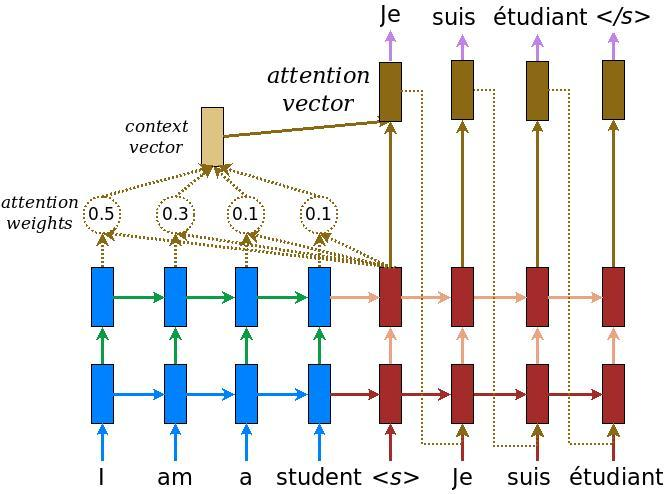
\includegraphics[width=6cm]{pres_imgs/attention_mechanism}
  \caption{\label{fig:attention_mechanism} An NMT model with attention (Bahdanau, 2016). }
\end{figure}
\end{frame}

%------------------------------------------------
\section{Zero-Shot Translation (Johnson, 2017)}
\begin{frame}
\frametitle{Motivation for Google Zero-Shot Translation (Johnson, 2017)}
Problem
\begin{itemize}
\item Each pair of languages requires an encoder-decoder pair $\Rightarrow$ space is $O(n^2)$ in number of languages $n$.
\item Google would like to support upwards of 100 languages with sometimes few to no sentence-to-sentence pairs. \pause
\end{itemize}
Solution
\begin{itemize}
\item Universal decoder and encoder for all language pairs.
\item Add an artificial token to the input sequence to indicate the required target language.\pause
$$\texttt{Hello, how are you? -> Hola, ¿cómo estás?}$$
$$\texttt{<2es> Hello, how are you? -> Hola, ¿cómo estás?}$$
\end{itemize}
\end{frame}

\begin{frame}
\frametitle{Zero-Shot Architecture}
 \begin{figure}
  \centering
  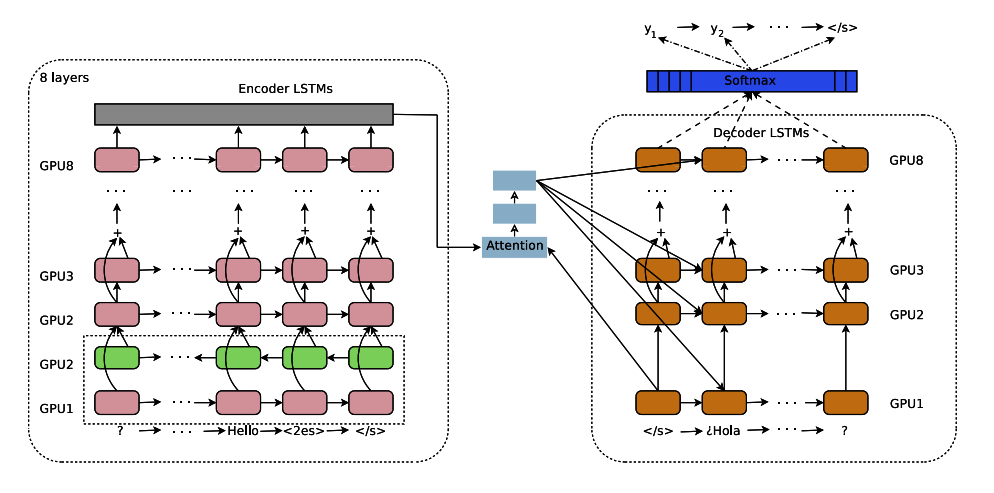
\includegraphics[width=10cm]{pres_imgs/zero_shot_arch}
  \caption{\label{fig:zero_shot_arch} Google Zero-Shot Architecture (Johnson, 2017). Source sentence is reversed and prepended to the target language token.}
\end{figure}
\end{frame}

\begin{frame}
\frametitle{Results}
\begin{itemize}
\item On the many-to-many task, the model underperforms production translation models by 2.5\%.
 \begin{figure}
  \centering
  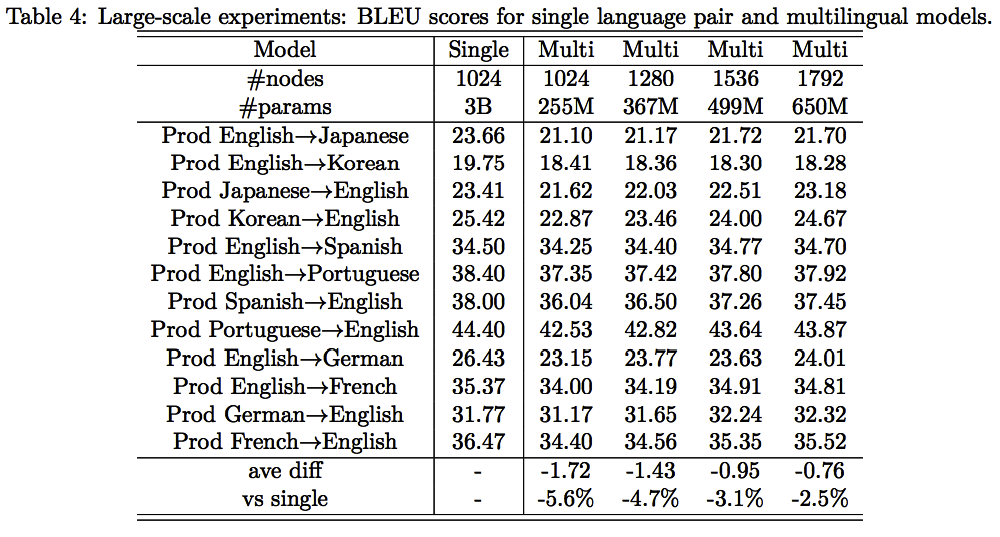
\includegraphics[width=8cm]{pres_imgs/manyto-many}
  \caption{\label{fig:manyto-many} When trained on all pairs of three languages, the model achieves comparable BLEU scores. Since the simplest model has 255$M$ instead of 3$B$ parameters, this result is satisfying.}
\end{figure}

\end{itemize}

\end{frame}

\begin{frame}
\frametitle{Zero-Shot}
The model can translate between languages for which there was no parallel data during training.
 \begin{figure}
  \centering
  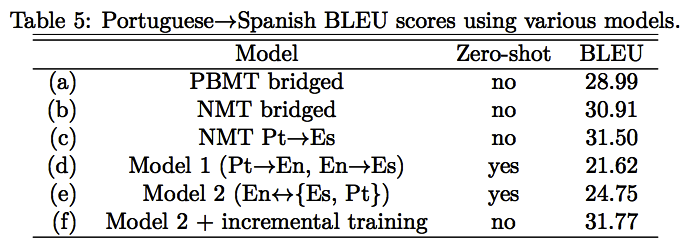
\includegraphics[width=8cm]{pres_imgs/zeroshottab}
  \caption{\label{fig:zeroshottab} PBMT is a phrase based translation system. NMT bridged is translation from Portuguese to Spanish going through English. NMT Pt$\rightarrow$Es is a standard NMT model with attention trained on all available Portuguese to Spanish sentences. Model (f) is trained on a tenth of the data of model (c).}
\end{figure}
\end{frame}

\begin{frame}
\frametitle{Interlingua}
\begin{columns} % The "c" option specifies centered vertical alignment while the "t" option is used for top vertical alignment

\column{.5\textwidth} % Left column and width
\textbf{Source Language Code-Switching}
What if we mix languages in the source sentence?
 \begin{figure}
  \centering
  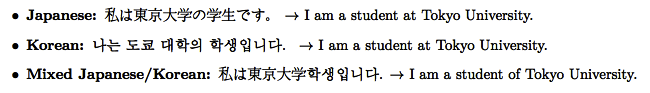
\includegraphics[width=\textwidth]{pres_imgs/srcswitch}
  \caption{\label{fig:srcswitch} The model handles mixed input language no problem.}
\end{figure}

\column{.5\textwidth} % Right column and width
\textbf{Weighted Target Language Selection}
What if we feed linear combinations of target tokens?
 \begin{figure}
  \centering
  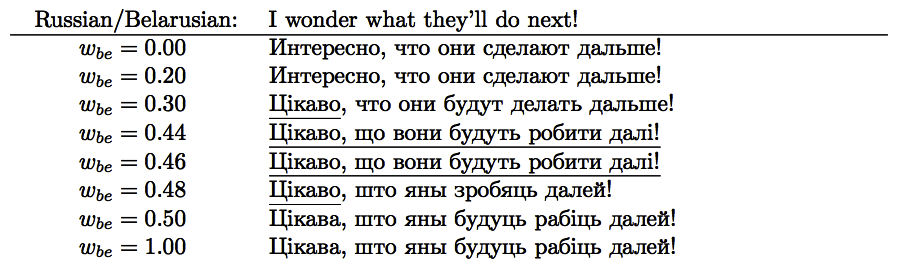
\includegraphics[width=\textwidth]{pres_imgs/trgswitch}
  \caption{\label{fig:trgswitch} The model translates into Ukrainian in the process of translating to Russian and Belarusian.}
\end{figure}
\end{columns}
\end{frame}

\begin{frame}
\frametitle{Interlingua}
 \begin{figure}
  \centering
  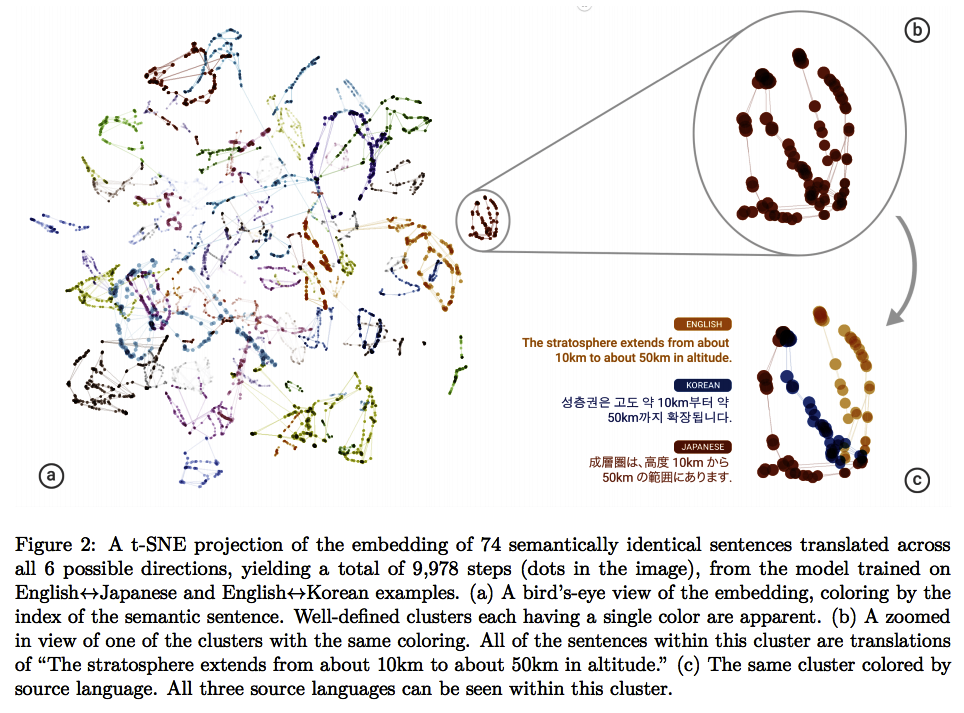
\includegraphics[width=.75\textwidth]{pres_imgs/zeroshotlatent}
  \caption{\label{fig:zeroshotlatent} Semantically identicle sentences have similar encodings.}
\end{figure}
\end{frame}

%------------------------------------------------
\section{Unsupervised Neural Machine Translation (Artetxe, 2018)}
\begin{frame}
\frametitle{UNMT Motivation}
\begin{itemize}
\item \textbf{Question} How well can we translate between language $l_1$ and $l_2$ given a corpus of text $X_1$ of language $l_1$ and a corpus of text $X_2$ of language $l_2$?\\
$$\rightarrow \text{Strong baseline for supervised NMT}$$
$$\rightarrow \text{Translation in low-resource contexts}$$
\pause
\item \textbf{Solution} Train universal encoder and language-specific decoders to denoise and backtranslate.\\\pause
This solution is one of many proposed solutions to this problem.
\end{itemize}
\end{frame}

\begin{frame}
\frametitle{Model}
 \begin{figure}
  \centering
  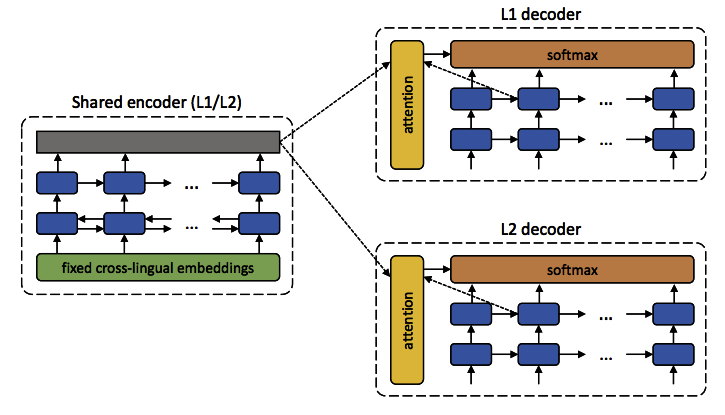
\includegraphics[width=.8\textwidth]{pres_imgs/unsupmodel}
  \caption{\label{fig:unsupmodel} At test time, a sentence $src$ from either $l_1$ or $l_2$ is fed to the encoder, and the target sentence decoder is used to predict a translation. At training time, the decoder used is the decoder associated with the language of $src$.}
\end{figure}

\end{frame}

\begin{frame}
\frametitle{2 ``Differences" from Standard NMT}\pause
\begin{itemize}
\item \textbf{2-step training} Cross-lingual word embeddings are determined in an initial training step (Johnson, 2017). These embeddings are then frozen before training the encoder-decoder system. \pause
\item \textbf{L$_{denoise}$ + L$_{backtranslate}$} Training the ecoder-decoder consists of a loss associated with the ability to back-translate and a loss associated with the ability to denoise.
\end{itemize}
\end{frame}

\begin{frame}
\frametitle{L$_{denoise}$}
\textbf{Loss}\\
Given a sequence of length $N$, make $N/2$ transpositions iteratively. The model is trained with the standard word-by-word loss. Let $C(x)$ return our noise model applied to sentence $x$.
$$ L_{denoise} = \mathbb{E}_{x\sim X_l, \hat{x}\sim d(e(C(x)),l)}\Delta(\hat{x},x) $$
An example denoising case
$$\texttt{\small this is example an sentence denoising for presentation my}$$
$$\texttt{\small -> this is an example denoising sentence for my presentation}$$
\end{frame}

\begin{frame}
\frametitle{L$_{backtranslate}$}
Given an input sentence in one language, use the system in inference mode with greedy decoding to translate it to the other language. In this way, we obtain pseudo-parallel sentence pairs. Let $x'=d(e(x),l')$.
$$ L_{backtranslate} = \mathbb{E}_{x\sim X_l, \hat{x}\sim d(e(x'),l)}\Delta(\hat{x},x) $$
In the semi-supervised model, we also mix in parallel sentence examples to this loss. The above loss has had some success in unsupervised image-to-image translation (Zhu, 2018).\\ \pause
\begin{figure}
  \centering
  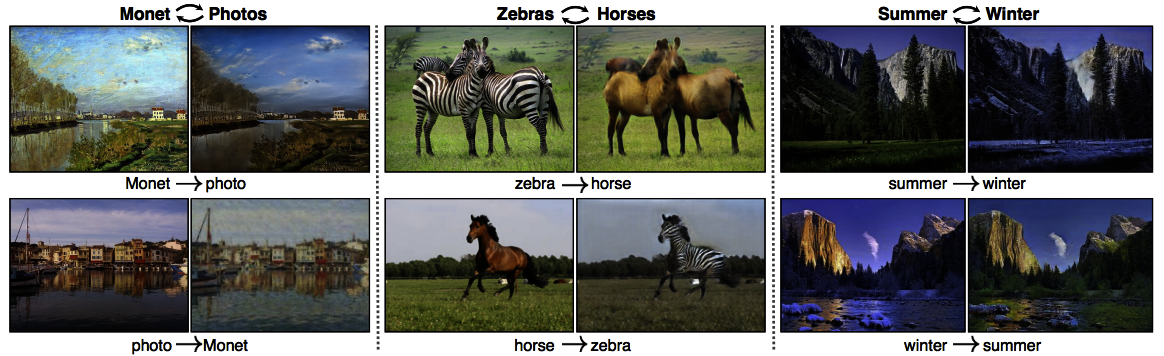
\includegraphics[width=\textwidth]{pres_imgs/imagetran}
%  \caption{\label{fig:imagetran} The model performs ``surprisingly" well. However, there is discussion of whether this model is actually interesting given the lack of success of models 7., 8., and 9. in a fully supervised setting.}
\end{figure}
\end{frame}

\begin{frame}
\frametitle{Evaluation}
\textbf{Details}
\begin{itemize}
\item French-English and German-English datasets from WMT 2014.\pause
\item \textbf{Unsupervised model} trained on News Crawl corpus articles from 2007 to 2013.\pause
\item \textbf{Semi-Supervised model} Additional 10k or 100k random sentence pairs from News Commentary.\pause
\item \textbf{Supervised model} WMT 2014 $+$ UN and Gigaword corpus for French-English.\pause
\item Spanish-English WMT data used for hyperparameter exploration.\pause
\item Frozen cross-lingual embeddings from Artetxe (2017).
\end{itemize}
\end{frame}

\begin{frame}
\frametitle{Results}
 \begin{figure}
  \centering
  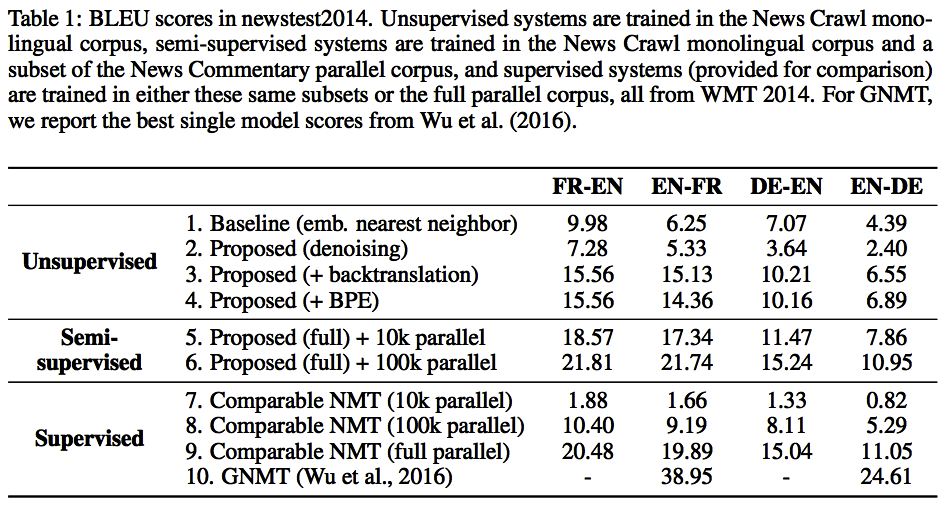
\includegraphics[width=.9\textwidth]{pres_imgs/unsupresults}
  \caption{\label{fig:unsupresults} The model performs ``surprisingly" well. However, there is discussion of whether this model is actually interesting given the lack of success of models 7., 8., and 9. in a fully supervised setting.}
\end{figure}
\end{frame}

\begin{frame}
\frametitle{Evaluation}
 \begin{figure}
  \centering
  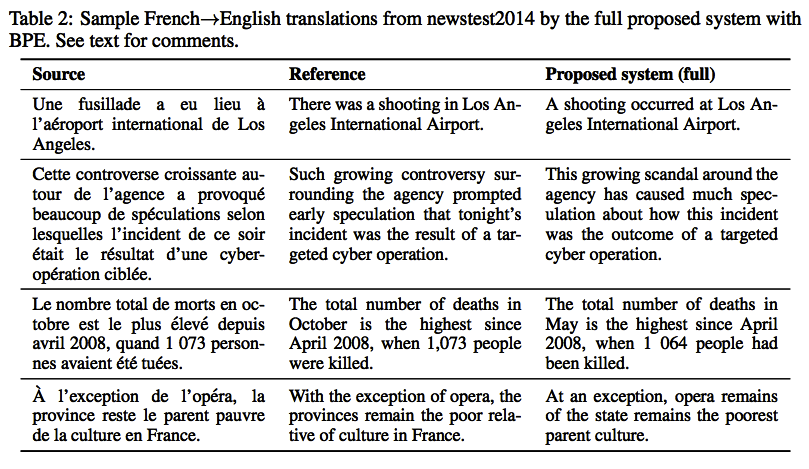
\includegraphics[width=.9\textwidth]{pres_imgs/unsupfrench}
  \caption{\label{fig:unsupfrench} Example translations for the best unsupervised model. The model is a decent translator.}
\end{figure}
\end{frame}
%------------------------------------------------
\begin{frame}
\frametitle{Extension Ideas AKA Pipe Dreams}
We want to enforce that given a source sentence $src$, the translation $M(src)$ has the same meaning as $src$ and is indistinguishable from sentences in the corpus of the target language.\\ \pause
~\\
\textbf{Problem} Translations $M(x_{src})$ indistiguishable from corpus $x_i \sim X_{tgt}$\\ \pause
$\Rightarrow$ \textbf{L$_{adversary}$} Force translations to fool a discriminator\\ \pause
~\\
\textbf{Problem} Translations $M(x_{src})$ should capture the meaning of $x_{src}$\\ \pause
$\Rightarrow$ \textbf{L$_{back^n translate}$} force invertibility of $M$ over $n$ cycles between $l_{src}$ and $l_{tgt}$.\\ \pause
~\\
\textbf{Problem} Words aren't well defined for certain languages\\ \pause
$\Rightarrow$ Add a language model loss with word-pieces to train end-to-end (Wu, 2016)\\
\end{frame}


%------------------------------------------------
%------------------------------------------------



%------------------------------------------------



%------------------------------------------------



%------------------------------------------------



%------------------------------------------------


%------------------------------------------------


%------------------------------------------------

\begin{frame}
\Huge{\centerline{The End. Questions?}}
\end{frame}

%----------------------------------------------------------------------------------------

\end{document}